\documentclass[10pt,a4paper,english,onecolumn]{IEEEtran}

\usepackage{datetime}
\usepackage{caption}
\usepackage{graphics}
\usepackage{graphicx}
\usepackage{minted}
\usepackage[utf8]{inputenc}
\usepackage[
    backend=bibtex,
    style=numeric,
    bibencoding=ascii,
    sorting=ynt
]{biblatex}
\addbibresource{resources}

\renewcommand*\contentsname{Table of Content}
\renewcommand*\listfigurename{List of Images}
\renewcommand\listingscaption{Example}
\renewcommand{\listtablename}{List of Tables}
\captionsetup[table]{name=Table}
\renewcommand*\figurename{Image}
\usemintedstyle{bw}
\hyphenpenalty=100000
\nocite{*}

\begin{document}

\title{Dynamic Taint Analysis}

\author{Ioana BRĂNESCU$^{1}$, Andreea-Larisa COZUC$^{2}$, Andreea-Diana OLTEAN$^{3}$, and George-Andrei IOSIF$^{4}$\\
$^{1,2}$\emph{Politehnica University of Bucharest, Computer Science Department, Romania}\\
Email: $^{1}$ioana.branescu0601@stud.acs.upb.ro, $^{2}$andreea.cozuc@stud.acs.upb.ro, $^{3}$andreea.oltean0208@stud.acs.upb.ro $^{4}$george\_andrei.iosif@stud.acs.upb.ro}

\maketitle

\begin{abstract}

Three papers on dynamic taint analysis (both online and offline) are examined independently in this essay. Furthermore, their strengths and weaknesses are highlighted, and comparisons between them are used to argue our point of view. At the end of the essay, additional approaches and techniques that have been successfully integrated with dynamic taint analysis, to improve its accuracy and performance, are presented. 

\end{abstract}

\section{Introduction}

As we are living in the era of information, the security of information systems is gaining more and more attention. An attacker needs only one vulnerability, which, once exploited, can have a devastating effect on the whole system. Given the increasingly huge number of threats and the size of the modern infrastructures, \textbf{manual security assessments are no longer viable}, and the process had to be automated.

\subsection{Automated Vulnerability Assessment}

There are various approaches when it comes to automated vulnerability detection, and they mainly fall in one of the following categories:

\begin{itemize}
    \item \textbf{Fuzzing}: It involves feeding the program with massive amounts of random inputs, including invalid and unexpected ones. If the program crashes for a certain input, the cause can be investigated. Even if this technique does not provide false positives, and it is very useful for finding bugs which were missed during manual testing, it takes a lot of time, and it is becoming more and more inefficient for the vulnerability detection of modern software.
    \item \textbf{Symbolic execution}: It uses symbolic values instead of concrete values as program inputs, and represents the values of program variables as symbolic expressions of those inputs. Even if, theoretically, it can find all the possible execution paths of the program and solve constraints for each of them, it's not applicable to complex, real world programs due to path explosion.
    \item \textbf{Taint analysis}, which is going to be further presented in detail.
\end{itemize}

\subsection{Taint Analysis}

The main idea of taint analysis consists of defining a taint source (untrusted, like user input data or network data), marking the data coming from that source as taint and detecting whether it is further used in dangerous ways or if it influences other pieces of data which are used in dangerous ways. Basically, \textbf{any data coming from an outsider represents a potential risk} which has to be monitored.

\begin{itemize}
    \item \textbf{Static taint analysis}: It works mainly at source code level by means of abstract interpretation techniques. It has a higher coverage and better analysis efficiency, but it needs access to the source code, which isn't available in many cases.
    \item \textbf{Dynamic taint analysis}: It has better accuracy, and most importantly, it doesn't need the application's source code, so is the more commonly used approach. It can be done in \textbf{online mode} (the analysis is executed at runtime, accompanied by the execution of the program and once the program stops, the analysis also stops) or in \textbf{offline mode} (the trace of program execution is recorded into files and the analysis is performed based on them).
\end{itemize}

Further, we are going to analyse and compare three papers which are presenting different tools and approaches based on \textbf{dynamic taint analysis}:

\begin{itemize}
    \item "\textit{Dynamic Taint Analysis for Automatic Detection, Analysis and Signature Generation of Exploits on Commodity \\Software}" \cite{taintcheck};
    \item "\textit{SwordDTA: A Dynamic Taint Analysis Tool for Software Vulnerability Detection}" \cite{sworddta}; and
    \item "\textit{OFFDTAN: A New Approach of Offline Dynamic Taint Analysis for Binaries}" \cite{offdtan}.
\end{itemize}

\section{Description of the Proposed Solutions}

\subsection{TaintCheck}

This paper is the oldest of the ones analysed in this essay (published in 2005) and it presents one of the first tools which uses dynamic taint analysis, called \textbf{TaintCheck}. The author's motivation was building a vulnerability detector that produces a very small number of false positives (meaning that once a problem is detected, that problem is for sure a real one), is able to provide detailed information about the vulnerability and exploit and doesn't require source code or specially recompiled binaries (so it could be used for analysing commodity software).

The main idea the authors are building on is that an attack is provoked by altering some data (sometimes legitimate) with data provided by the attacker. Based on this approach, TaintCheck can detect \textbf{overwrite attacks} that cause a sensitive value (such as return addresses, function pointers, and format strings) to be overwritten with the attacker's data. Also, once an attack is detected the tool can automatically provide information about the vulnerability, about how it was exploited and about which part of the payload is actually used for exploitation. The last information can be further used to \textbf{generate signatures for attack filtering} , which are especially useful when we're talking about protecting a distributed environment. In this case, if a protected computer has been attacked, the signature is extracted and then shared with the others computers in the network.

There are two implementations of TaintCheck: the one the paper focuses on, which uses \textbf{Valgrind} and the other, which is designed for Windows, using \textbf{DynamoRIO}. The flow can be described like this: when a new basic block is reached, Valgrind translates it into UCode (RISC-like instruction set), which is then passed to TaintCheck, where the taint analysis code is incorporated. The rewritten UCode block goes back to Valgrind where it is translated back to x86 code, and it's then ready for execution. This mechanism also caches blocks for avoiding multiple translations.

The first step followed by TaintCheck is \textbf{overflow detection}:

\begin{itemize}
    \item \textbf{TaintSeed}: The main goal of this first step is \textbf{knowing which inputs are going to be tainted}. Depending on the policy the tool is set on, data coming from a file, network data or stdin data is going to be marked as tainted. Technically, each byte of memory (including the registers, the stack and the heap) has a four-byte shadow memory which stores a pointer to a Taint data structure if the location is tainted or a \mintinline{bash}{NULL} pointer otherwise. This taint data structure keeps a system call number, a snapshot of the current stack and a copy of the data that was written, which, in case of an attack, is going to be used by the Exploit Analyzer. Depending on the user's needs (mainly due to memory constraints), the logging option can be disabled and each byte is going to be shadowed only by a bit which shows whether the byte is tainted or not.
    \item \textbf{TaintTracker}: At this point, the tainted data is introduced, but we need to establish how it's going to \textbf{propagate} during the execution. This is going to happen due to data movement instructions like \mintinline{bash}{move}, \mintinline{bash}{push}, \mintinline{bash}{pop} (if the source is tainted, the destination is tainted too) or due to arithmetic instructions like \mintinline{bash}{add}, \mintinline{bash}{sub}, \mintinline{bash}{xor} (if one byte of the operands is tainted the result is also going to be tainted). Cases like \mintinline{bash}{xor eax, eax} or \mintinline{bash}{sub eax, eax} are handled, but more complex similar cases weren't resolved.
    \item \textbf{TaintAssert}: Now, the tainted data is already distributed in different places in memory, but we still need to \textbf{establish what kind of tainted data usage should raise an attack alarm}. This is going to be done through a seemingly simple approach, but which gave very good results when tested against real world exploits, like ATPhttpd exploit (a buffer overflow vulnerability, which is exploitable through a GET request which reads a very long filename which is actually a shellcode) or Slammer (buffer overflow vulnerability in MS-SQL Server which leads to a return address overwrite) and it gave zero false-positive during evaluation. There are four interesting places which are monitored for tainted data: jump addresses (namely \mintinline{bash}{jmp TAINTED}), format strings (namely \mintinline{bash}{printf(TAINTED)}), system call arguments (namely \mintinline{bash}{syscall(TAINTED)}) and application or library-specific checks (namely \mintinline{bash}{libcall(TAINTED)}).
\end{itemize}

If TaintAssert detected something, \textbf{Exploit Analyzer} kicks in and based on the data kept in Taint data structures it does a backtracking for finding out exactly which byte of the payload is responsible for the overwrite and how it got to that place in memory.

\begin{center}
    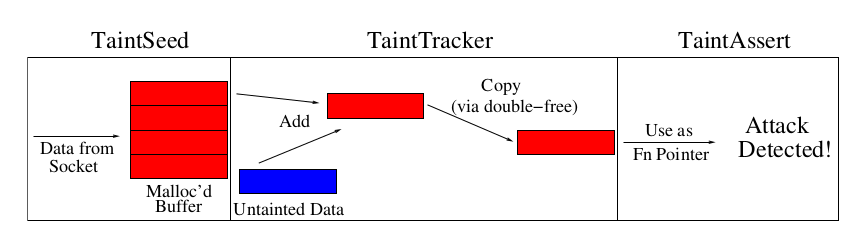
\includegraphics[width=12cm]{images/taintcheck.png}
    \captionof{figure}{The Architecture of TaintCheck}
    \vspace{0.5cm}
\end{center}

TaintCheck does a great job at detecting overwrite attacks, but when it comes to performance, things aren't so great anymore. Different programs were run with the detector active and the \textbf{running time for the same job was affected a lot} (sometimes with 36x - anyway, when the article was written the tool was in the research phase, so performance wasn't the main focus).

The tool presented until this point can prevent and detect attacks on individual sites, but with a \textbf{significant overhead} , which makes it hard for the tool to be used in large infrastructures. Also, even if individual protection is great, it would be ideal to have a tool which can provide protection on all of one's services, at network level, with a low performance overhead. For achieving this goal, an optimised implementation is further presented, called the \textbf{Hybrid Exploit Detector}.

The main idea of this hybrid detector is that there is going to be a new component, called \textbf{trace logger} which is going to log the recent traffic. After that, a flow selector will pick only some flows based on a set of rules and in the end, the selected flows will be evaluated by TaintCheck (obviously, this is going to decrease the performance impact). The rules used in selection are:

\begin{itemize}
    \item Any flow is going to be randomly selected with a probability of at least $ P $, which is a parameter.
    \item Some suspected flows are going to be selected. In this case, the selection is going to be made based on heuristics like:
        \begin{itemize}
            \item Flows that are sent from sources that have been performing port scans.
            \item Flows that contain executable code.
            \item Flows with strange byte patterns that are suddenly very common.
            \item Flows that are sent to honeypots.
    \end{itemize}
\end{itemize}

The last heuristic is a fascinating one, as it was also used during testing (the tool was \textbf{tested on Carnegie Mellon's honeypots network, and} it caught real attacks like SQL Slammer). A honeypot is a network resource which looks like a real computer system, but is actually used for fooling cybercriminals into thinking it's a legitimate target (the honeypots might have deliberate security vulnerabilities) so new attacks can be discovered and analysed. Given the fact that honeypots are technically traps which are supposed to be targeted by many attackers, it's understandable why it would be useful to check the flows directed to such a server with TaintCheck.

If we want to \textbf{prevent attacks in a distributed fashion} (not just log the flows, execute them normally and then reply some of them with TaintCheck on), we can redirect the suspected flows to an isolated server where they are going to be analysed, but this might not always be a good idea because, due to the performance impact the detector has on the execution time, the protected server might respond too slowly to the request, the attacker might realise that he was detected, and he could stop targeting us and move on to an unprotected target. To avoid this unpleasant situations, we could leave the flows run normally on all the machines, redirect the suspected flow to the protected server (which runs TaintCheck), and if an attack is discovered, we could quarantine the initially attacked server, \textbf{generate the attack's signature} and distribute it to the rest of the unprotected servers which are going to further filter the requests based on the received signature.

But how are these signatures automatically generated? The techniques used at that time were treating payloads as opaque byte sequences and attempting to find patterns that are constant across the attack payload (an approach which needed a lot of payload samples). With TaintCheck, we are able to identify exactly which value in the original flow overwritten a return address or a function pointer, and the determined signature will usually consist only of the most significant three bytes. It was empirically proved that this length is enough for detection of numerous exploits, for both code injection and code reuse attacks.

\subsection{SwordDTA}

Published in 2016, this paper doesn't provide as many details as the previous one. Still, there are four types of vulnerabilities which are detected by SwordDTA:

\begin{itemize}
    \item \textbf{Buffer Overflow}: Occurs when a program attempts to put more data in a buffer than it can hold. It is usually associated with dangerous functions like \mintinline{bash}{strcpy}, \mintinline{bash}{strcat}, \mintinline{bash}{sprintf}, \mintinline{bash}{vsprintf}, \mintinline{bash}{gets}, \mintinline{bash}{scanf} and comes from a bad sanity check of user-input data.
    \item \textbf{Integer Overflow}: Occurs when an integer which isn't properly sanitised is used in determining an offset or size for a memory operation (allocation, copying, concatenation). It typically leads to crashes, but in some cases it can lead to buffer overflow and even arbitrary code execution.
    \item \textbf{Division by zero}: Occurs when an unexpected value is provided to the application.
    \item \textbf{Use-after-free}: Frequently used for exploiting web browsers, can lead to many problems, from data corruption to arbitrary code execution.
\end{itemize}

\textbf{SwordDTA} is implemented via \textbf{Pin DBI} (abbreviation of dynamic binary instrumentation). This framework was chosen due to the fact that Pin supports four operating systems: Windows, Linux, OSX and Android and four architectures: 32-bit x86, 64 bit x86, Itanium and ARM. The detector currently runs on 32-bit x86, and it is written in C++, but the authors are planning on extending the functionalities to Windows and x96-64. Also, Pin is efficient and the option of using it claims to minimise the slow execution problem the dynamic taint analysis usually suffers from.

The steps followed by SwordDTA are:

\begin{enumerate}
    \item \textbf{Taint Introduction}: The first step is to \textbf{specify what data to be treated as tainted}. This can happen any time during the execution of the program. A function is called to tag a number of successive memory addresses as taint. The tool supports four kinds of taint source: \textbf{file, standard input} , \textbf{memory} and \textbf{network packet}.
        \begin{itemize}
            \item For file taint source, SwordDTA hooks file related system calls. It first hooks the "open" system call and whenever a file is open, it checks if the open file is what we want to track. SwordDTA can take part of all the bytes of an input file as taint source.
            \item For standard input taint source, SwordDTA uses the Pin API to get the user-input command line arguments at the beginning of a new thread.
            \item For memory taint source, the SwordDTA will set the block of memory that was specified as taint source (usually used to detect use after free vulnerabilities).
            \item For network packet taint source, SwordDTA hooks socket-related system calls.
        \end{itemize}
    \item \textbf{Taint Propagation}: The next step is to track the propagation of taint sources and \textbf{mark all the data affected by a taint source as tainted data}. There are two problems: taint propagation granularity and the size of taint tag:
        \begin{itemize}
            \item \textbf{Taint propagation granularity} refers to the smallest taint unit to be tracked. If it is too large it would lead to tainted data loss and inaccuracy, while the small granularity would lead to excessive taint proliferation (in the paper the granularity is set to one byte).
            \item Larger \textbf{tags} are more versatile as they allow for different types of data to be tagged uniquely. However, larger tags require more complicated propagation logic and space (in the paper, they use single bit tags). As there are two objects that can get tainted, memory locations and registers, the tool stores taint tags in a data structure called \mintinline{bash}{mem_taint_map} for the first one and in another data structure called \mintinline{bash}{reg_taint_map} for the second one. Also, for each memory block a bitmask is used to decide whether the data is tainted or not.
        \end{itemize}
    \item \textbf{Vulnerability Detection}: For each type of detected vulnerability, SwordDTA \textbf{decides whether to trigger an alarm} or not based on the following rules:
        \begin{itemize}
            \item For buffer overflow, it checks the parameters of dangerous functions such as \mintinline{bash}{memcpy}.
            \item For integers overflow, it checks the parameters of memory allocation functions (\mintinline{bash}{malloc} and \mintinline{bash}{calloc}).
            \item For division by zero, it instruments the div and \mintinline{bash}{idiv} instructions.
            \item For use after free, it sets the freed memory as taint source and checks whether there is any operation performed on that memory zone afterwards. If that given memory zone is reallocated by \mintinline{bash}{malloc}, it is cleared from the tainted data sources.
        \end{itemize}
\end{enumerate}

\begin{center}
    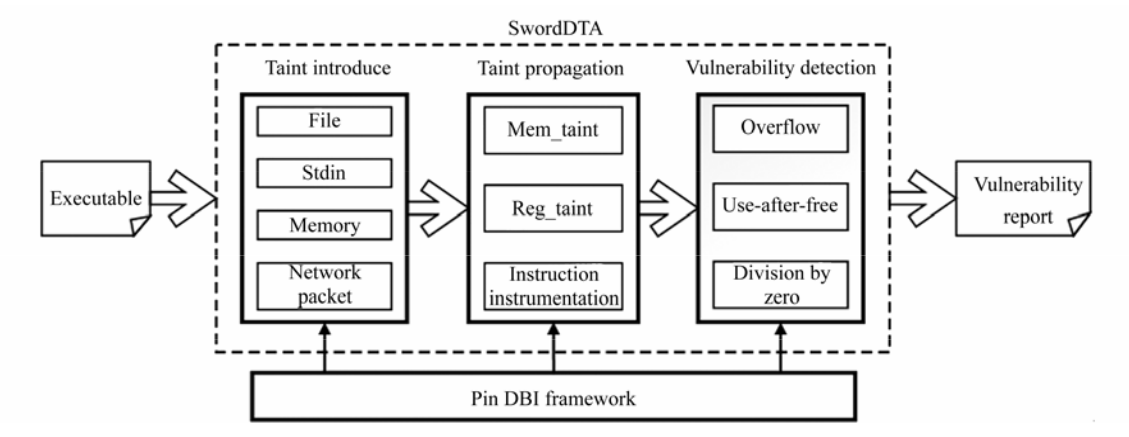
\includegraphics[width=12cm]{images/sworddta.png}
    \captionof{figure}{The Architecture of SwordDTA}
    \vspace{0.5cm}
\end{center}

When it comes to evaluation and case studies, SwordDTA is evaluated based on both textbook attacks and 11 real world attacks from each of the four categories pointed out earlier, and it passes all of them.

\subsection{OFFDTAN}

This is the newest of the analysed papers, as it was published in 2018. OFFDTAN is an instrument for \textbf{dynamic taint analysis}. Similar to the previously presented papers, OFFDTAN works based on the idea of tracking taint data and checking whether it gets in dangerous places or not.

A remarkable aspect about this software is that it uses an \textbf{offline approach} to discover the exploited vulnerabilities by replaying the execution using the recorded information from the log files. On the other hand, it uses \textbf{KVM virtualization on QEMU} , running in an environment isolated from the host operating system.

The steps followed by \textbf{OFFDTAN} are:

\begin{enumerate}
    \item \textbf{Dynamic information acquisition}: In this stage, the trace of program execution and the taint source log are \textbf{dynamically captured} in order to be further used for the offline analysis. The program execution trail is recorded using the runtime informations, which consists of \textbf{processor's state} (including general registers, flag registers, segment registers and control registers), \textbf{memory information} and \textbf{process information} (in the Windows operating system, kernel data structures are used). In the OFFDTAN approach, in order to mark taint sources, the parameters and return values of the system services responsible for reading input data will be monitored. As a consequence, the record about taint data keeps the offset in the taint source file, the length and the memory head location.
    \item \textbf{Vulnerability modelling}: OFFDTAN detects two types of vulnerabilities: stack buffer overflow and controlled jumps. When it comes to buffer overflows, the model is concerned about monitoring the ebp register and the return addresses that might hijack the control flow of the program. In the controlled jump vulnerability model, the tool checks the integrity of the jump's destination.
    \item \textbf{Offline analysis}: Offline analysis stage loads the trace file of program execution and taint source log file to perform offline analysis on the basis of taint propagation policy and vulnerability checking strategy. This is divided in 3 stages:
        \begin{itemize}
            \item \textbf{Program virtual replaying}: By loading instructions and contexts recorded by the trace file simulate program execution according to the order of instruction.
            \item \textbf{Dynamic taint analysis}: Performs taint analysis during virtual replaying by loading a taint source log file. Propagation policy is used to guide this analysis.
            \item \textbf{Program vulnerability analysis}: Checks the program vulnerabilities guided by security policy.
        \end{itemize}
    \item \textbf{Backtrace analysis}: In this step, the program is executed backwards by using the journal files of the execution (vulnerability log file and taint propagation flow graph) and, in this way, the source of tainted data is determined.
\end{enumerate}

The above-mentioned dynamic taint analysis step consists in:

\begin{itemize}
    \item \textbf{Taint Data Recording}: Offline analysis, unlike standard dynamic taint analysis, adds taint source by evaluating the taint source log file. The taint source information with the same number would be stored into the taint state space according to the virtual replaying instruction number. The taint status of memory addresses and registers is recorded in the taint state space.
    \item \textbf{Taint Propagation Policy}: Propagation policy describes how taint data should be propagated during program replaying and it is constructed after many program tests.
    \item \textbf{Constructing Taint Propagation Flow Graph}: OFFDTAN evaluates the effect of each instruction based on the propagation policy and the operand's taint state space, and then constructs a taint propagation flow graph with instruction nodes.
\end{itemize}

\begin{center}
    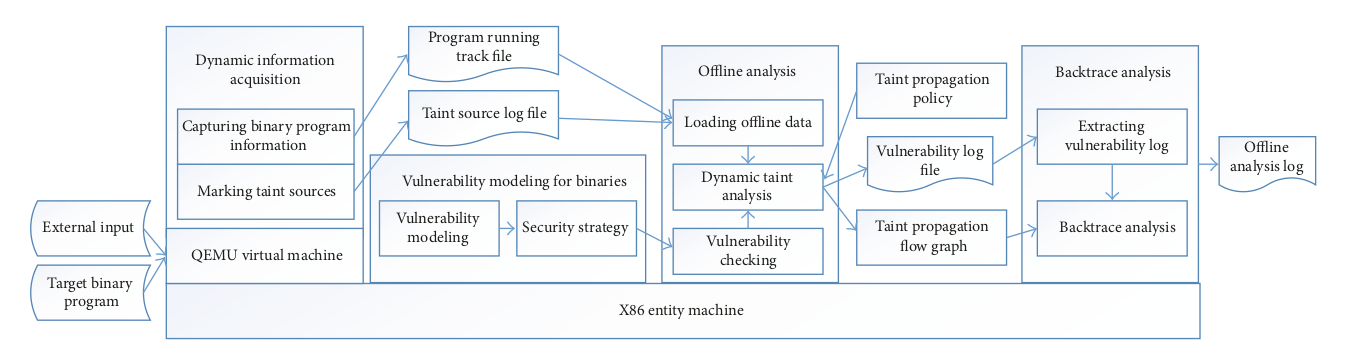
\includegraphics[width=12cm]{images/offdtan.png}
    \captionof{figure}{The Architecture of OFFDTAN}
    \vspace{0.5cm}
\end{center}

During evaluation, the tool was tested against six large applications, including FeiQ 2.5 and Word 2010. It turned out the tool can correctly determine what caused the program's crashes and at which offset the problem appeared.

\section{Comparative Analysis}

The descriptions above give a factual glimpse into the binary analysis through dynamic tainting, as seen in the cited papers. In this chapter, we carry out an analysis on this approach of finding vulnerabilities in binaries and these papers, by determining what are their strengths and weaknesses and by comparing against each other.

\subsection{Strengths}

One of the most interesting methods we saw is the \textbf{translation from binary code into Assembly or UCode} , as approached in OFFDTAN and TaintCheck. This transformation from the machine code into another, higher level language, reduced the instructions whose functionality needed to be understood and ease the instrumentation process. At the same time, another advantage was that the malicious activity of the binary was detected at this low enough level, unlike SwordDTA, which we will detail in the next section. For example, OFFDTAN has a built-in vulnerabilities model to detect stack buffer overflow by watching the effect of a \mintinline{bash}{ret movsd} instruction to not alter important stack values such as the return address or the old stack base pointer.

A different approach was used in TaintCheck, where the translation into UCode lets the specific component detect attacks in a more intuitive manner: at the time when the tainted data is used. This contradicts the classic method in which dynamic taint analysis tools were implemented at that time, representing a main contributor to performance (besides the \textbf{caching mechanism} that ensured that the most frequent instructions were not instrumented multiple times) and to the \textbf{null false positive rate} that TaintCheck obtained. The latter is essential because unnecessary analyses of programs by security researchers are avoided, reducing the manual work that needs to be involved.

From an explanation point of view, we considered that SwordDTA is the best example. In the evaluation chapter, the authors of the papers offer a \textbf{case study} with a straight-forward program that encapsulated a buffer overflow vulnerability with inputs read from the file system. By detailing the analysis through the lens of each major component and offering output examples (mainly content of the log files, with program traces and detections), the whole functioning, motivations and architecture can be better understood by the reader of the paper.

The last innovative improvement that needs to be mentioned is the usage of \textbf{distributed techniques} in the proposed solutions to better and quickly detect attacks. It can be seen in the TaintCheck architecture that two different methods were used. First, to ensure a low reduction of the system performance, TaintCheck uses a two-tiered approach: suspicious networks flows are selected via two heuristics (one random, one based on intrusion detection systems heuristics) to be sent to the second tier, where they are run against a TaintCheck-protected server. At the same time, the remaining, supposedly clean flows are sent to an unprotected server. By averaging the response times (one larger, when the request is run against the protected server, and the other, smaller), it was seen that the perceived clients delays are minimal. On the other hand, if multiple TaintCheck \textbf{agents} are installed in one network, they \textbf{can communicate with each other} to share detections (via \textbf{generated signatures} ) and, in this manner, rapidly detect possible infections.

\subsection{Weaknesses}

We can see dynamic taint analysis as closely related to the control flow graph of a program, but data-oriented. By modelling the flow of the tainted information in the process, it can be determined if it alters some critical aspects of its functioning (such as execution flow and used data). This implies two major disadvantages: \textbf{the vulnerabilities are detected actively, on exploitation time} , and \textbf{the code coverage is dependent on the given input} (it does not explore exhaustively all execution paths).

Despite the above-mentioned advantages, we deduced weaknesses that can be easily patched by involving more resources, mainly more time allocated to research and development.

First, we concluded that \textbf{a skilled attacker could evade the proposed techniques}. In SwordDTA, the buffer overflow vulnerability model, that is implemented by intercepting relevant library and system calls (such as \mintinline{bash}{memcpy}), could be eluded by using memory-related Assembly instructions, such as \mintinline{bash}{mov} (besides a \mintinline{bash}{rep} one). This could produce, for example, a return instruction overwrite, and it will not be detected by the proposed software product.

OFFDTAN, due to the default configuration (that is, realistically, not frequently changed by the security analysts), will only detect attacks with tainted data from network packets. Therefore, an attacker could cause the program to write the payload into a file and read it later to trigger the attack (if possible). In this case, as the data comes from the file system, OFFDTAN will not mark it as tainted and will not correctly detect the presumed attack.

Another common denominator for OFFDTAN and SwordDTA are the \textbf{small sizes of the test cases} that they use for evaluation. For instance, the latter uses only 15 programs, from which 4 of them were handmade by the researchers. Although the proposed solutions were able to detect the attacks, we consider that a conclusion was prematurely taken.

From a performance point of view, the two papers mentioned above \textbf{do not offer an absolute evaluation} of the effects on the host systems (only relative ones, in comparison to other solutions). Only TaintCheck shows that the computationally-intensive applications (archive creation ones) are \textbf{slowed down heavily} (up to a factor of 4). We consider that, even if this number is discouraging, their solution could be perfected if the emphasis is moved from research to development (especially to optimization techniques).

Lastly, SwordDTA and OFFDTAN were \textbf{closed source} , having an obvious disadvantage of not letting the community contribute to the projects. We found that TaintCheck was open source, but \textbf{discontinued} in 2018 (judging by the activity from the GitHub repository).

\section{Related Efforts}

The first two weaknesses mentioned in the above section, related to the dynamic taint analysis as a whole, could be solved by using another technique that has these as advantages: \textbf{fuzzing}. By giving specific inputs (generated via dummy, random approaches or via mutational or generational ones) to the program, the code coverage can be increased and so vulnerabilities can be detected proactively too \cite{fuzzy_dta}.

On the other hand, the performance overhead could be minimised by using the latest research in the \textbf{artificial intelligence} field (and achieving decent accuracy) \cite{neutaint} or speculative optimizations \cite{speculative_dta} to determine the instructions run next.

The last aspect that we think that could be improved is the scope of the analysis via dynamic tainting. As the papers described above refers only to vulnerabilities related to C programs (buffer overflows, use-after-free, integer overflows) and targets only a process at a time, we found indicators that there is ongoing research in \textbf{whole-system analysis} \cite{decaf++} and ones targeting \textbf{JavaScript} \cite{javascript_dta} and \textbf{Android} \cite{taintman}. This will increase the effects of using this technique to detect exploitation attempts on various platforms.

\section{Conclusions}

Finally, the three papers demonstrate the \textbf{utility} of dynamic taint analysis for discovering vulnerabilities during runtime, when attackers attempt to exploit the application, or offline, by using trace files generated by recording the process's behaviour.

Despite the fact that this technology has a \textbf{performance overhead} , as seen in the software solutions described above, we discovered that there is ongoing research to improve this aspect. On the other hand, we are optimistic that these, in addition to the new approaches and operating systems targeted by actual research, will make dynamic taint analysis \textbf{more accessible and performant}.

\section{Bibliography}
\nocite{*}
\printbibliography[heading=none]

\end{document}